\documentclass{math201}
\usepackage{hyperref}
\usepackage{bookmark}
\usepackage{minted}

% =============================================
% Part 0 信息
% =============================================

\mathsetup{
  % 学生姓名
  student = {某同学},
  % 学号
  student-id = {2021xxxx},
  % 院系
  experiment = {实验五 矩阵键盘输入控制实验},
  % 专业年级
  discipline = {集成电路设计与集成系统},
  % 日期
  date = {\today},
}

\begin{document}

% =============================================
% Part 1  封面
% =============================================

\makecover

% =============================================
% Part 2 主文档
% =============================================

\section{实验要求}

\begin{enumerate}
  \item 运行例程实验实验11 矩阵键盘输入+串口输出+LCD液晶显示,观察实验现象
  \item 看懂源程序
  \item 修改源程序,按下各个键时分别在串口和LCD液晶屏上显示如图所示符号
  \item 撰写实验报告、把修改的程序截图、实验现象的裁图或者图片整理到报告中
\end{enumerate}

\begin{figure}[H]
  \centering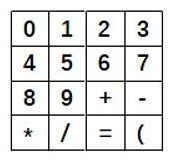
\includegraphics[width=0.6\linewidth]{requirements.jpg}
  \caption{实验要求}      
\end{figure}

\section{实验内容及结果}

\subsection{编写代码}

修改\texttt{main.c}文件,实现按下各个键时分别在串口和LCD液晶屏上显示如图所示符号。主要功能包括初始化LED、GPIO、LCD和串口通信。它还包括一个按键扫描功能,用于检测按键输入,并将按键值通过串口输出显示在LCD上。以下是代码的重要部分的简要说明:

\begin{enumerate}
  \item \texttt{LED\_GPIO\_Config()}:配置LED相关的GPIO。
  \item \texttt{GPIO\_Configuration()}:配置GPIO。
  \item \texttt{NT35510\_Init()}:初始化LCD显示。
  \item \texttt{Debu\_USART\_Config()}:配置调试用的串口。
  \item \texttt{NT35510\_GramScan(6)}:设置LCD显示模式。
  \item \texttt{Key\_scan()}:扫描按键输入并返回按键值。
  \item \texttt{LCD\_Test()}:用于测试LCD显示的函数。
\end{enumerate}

在\texttt{main}函数中,通过一个无限循环,不断调用\texttt{LCD\_Test()}和\texttt{Key\_scan()}函数,以及一个延时函数\texttt{Delay()}来实现连续的按键扫描和显示更新。

按键扫描函数\texttt{Key\_scan()}通过设置和重置GPIO位来检测哪个按键被按下,并将按键值存储在\texttt{key\_value}变量中,然后通过串口输出该值。每个按键对应一个字符,例如'0'到'9'、'+'、'-'、'*'、'/'、'='和'('。这些字符随后通过串口输出,并显示在LCD上。

\inputminted[
    frame=lines,
    framesep=2mm,
    baselinestretch=1.2,
    fontsize=\small,
    linenos
]{C++}{code/main.c}

\subsection{下载运行}

使用 \texttt{FlyMCU.exe} 下载程序到 STM32 开发版上,观察实验现象。

\subsection{实验现象}

\begin{figure}[H]
  \centering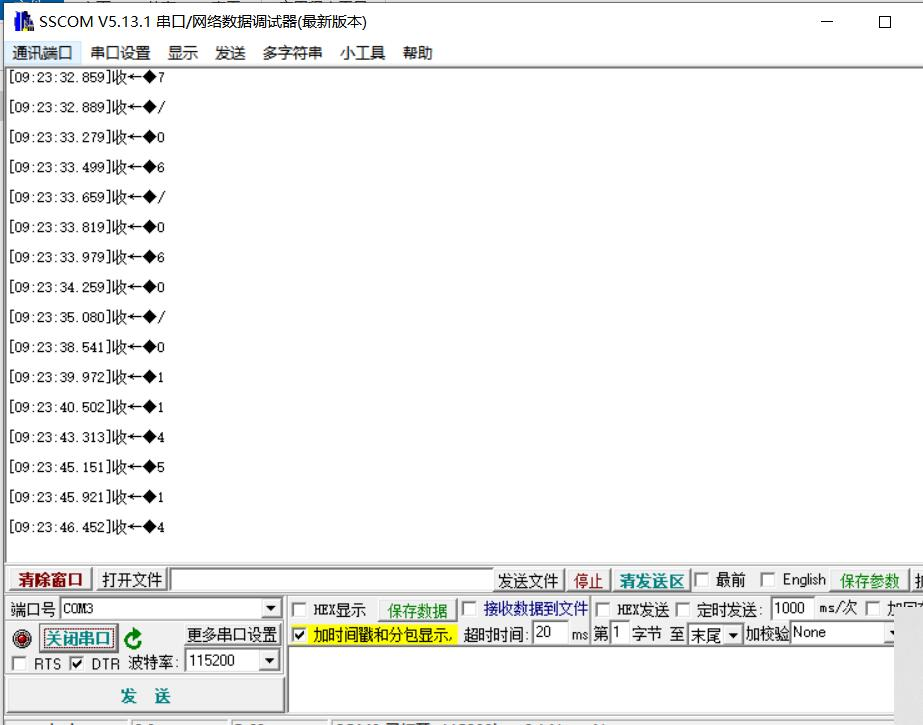
\includegraphics[width=0.6\linewidth]{result-com.jpeg}
  \caption{串口输出结果}
\end{figure}

\section{实验小结}

本次实验通过集成LED指示灯、按键输入、串口通信以及LCD显示,实验构建了一个交互式系统。系统能够响应用户的按键输入,并将结果实时显示在LCD屏幕上,同时通过串口输出相关信息。

\end{document}
